\textbf{Name:} \\

\medskip

\textbf{Conspirators:} 

\medskip
\medskip

\hrule

\medskip


%% \assignmentsonly{\pleasesubmitprojectdraft}

\begin{enumerate}

\item
  
  More on the peculiar nature of distributions of power law tails:
  
  Consider a set of $N$ samples,
  randomly chosen according
  to the probability
  distribution
  $P_{k} = c k^{-\gamma}$
  where
  $k = 1, 2, 3, \ldots$.

  %% (Note that $k$ is discrete rather than continuous.)
  %%   and $2 < \gamma < 3$.

  Estimate $\min k_{\rm max}$, the approximate minimum of 
  the largest sample in the system,
  finding how it depends on $N$.  

  (Hint: we expect on
  the order of 1 of the $N$ samples to have a value
  of $\min k_{\rm max}$ or greater.)
  
  \videohint{4tqlEuXA7QQ}{Some visual help on setting this problem up}

  We are just touching on the deep world of
  \wordwikilink{https://en.wikipedia.org/wiki/Extreme_value_theory}{extreme value theory.}
  Feel free to explore.

  
   \solutionstart

   %% solution goes here

   \solutionend

  Notes:
  \begin{itemize}
  \item
    For language, this scaling is known as Heaps' law (Stigler's Law applies again).
  \item
    In a later assignment, we will test this scaling
    by (thoughtfully) sampling from power-law size distributions.
  \end{itemize}
  
  
\item

  Code up Simon's rich-gets-richer model.
  
  Show Zipf distributions for $\simonalpha$ = 0.10, 0.01, and 0.001.
  and perform regressions to test
  $\alpha = 1 - \simonalpha$.

  Run the simulation for long enough to produce decent scaling
  laws (recall: three orders of magnitude is good).
  
  Averaging over simulations will produce cleaner results
  so try 10 and then, if possible, 100.
  
  Note the first mover advantage.

  
   \solutionstart

   %% solution goes here

   \solutionend

\item (3 + 3 + 3 points)
  For Herbert Simon's model of what
  we've called Random Competitive Replication,
  we found in class that the normalized number
  of groups in the long time limit, $n_{k}$, satisfies the following
  difference equation:
  \begin{equation}
    \label{eq:300.asn2nk}
    \frac{n_{k}}{n_{k-1}}
    =
    \frac{(k-1)(1-\simonalpha)}
         {1+(1-\simonalpha)k}
  \end{equation}
  where $k \ge 2$.
  The model parameter $\simonalpha$ is the probability
  that a newly arriving node forms a group
  of its own (or is a novel word, starts a new
  city, has a unique flavor, etc.).
  For $k=1$, we have instead
  \begin{equation}
    \label{eq:300.asn2n1}
    n_{1}
    =
    \simonalpha
    -(1-\simonalpha) n_{1}
  \end{equation}
  which directly gives us $n_{1}$ in terms of $\simonalpha$.

  \begin{enumerate}
  \item 
    Derive the exact solution for $n_{k}$ in terms
    of gamma functions and ultimately the
    beta function.  
  \item 
    From this exact form, determine
    the large $k$ behavior for $n_{k}$ ($\sim k^{-\gamma})$ and identify
    the exponent $\gamma$ in terms of $\simonalpha$.
    You are welcome to use the fact that
    $B(x,y) \sim x^{-y}$ for large $x$ and fixed $y$
    (use Stirling's approximation or possibly Wikipedia).
  \end{enumerate}

  Note: Simon's own calculation is slightly awry. 
  The end result is good however.
  
  %%  Some good news: in a burst of exuberance,
  %%  we outlined the derivation
  %%  in class on the board.
  %%  

  \videohint{OTzI5J5W1K0}{Setting up Simon's model}

  \assignmentsonly{
    The hint's output including the bits not in the video:\\
    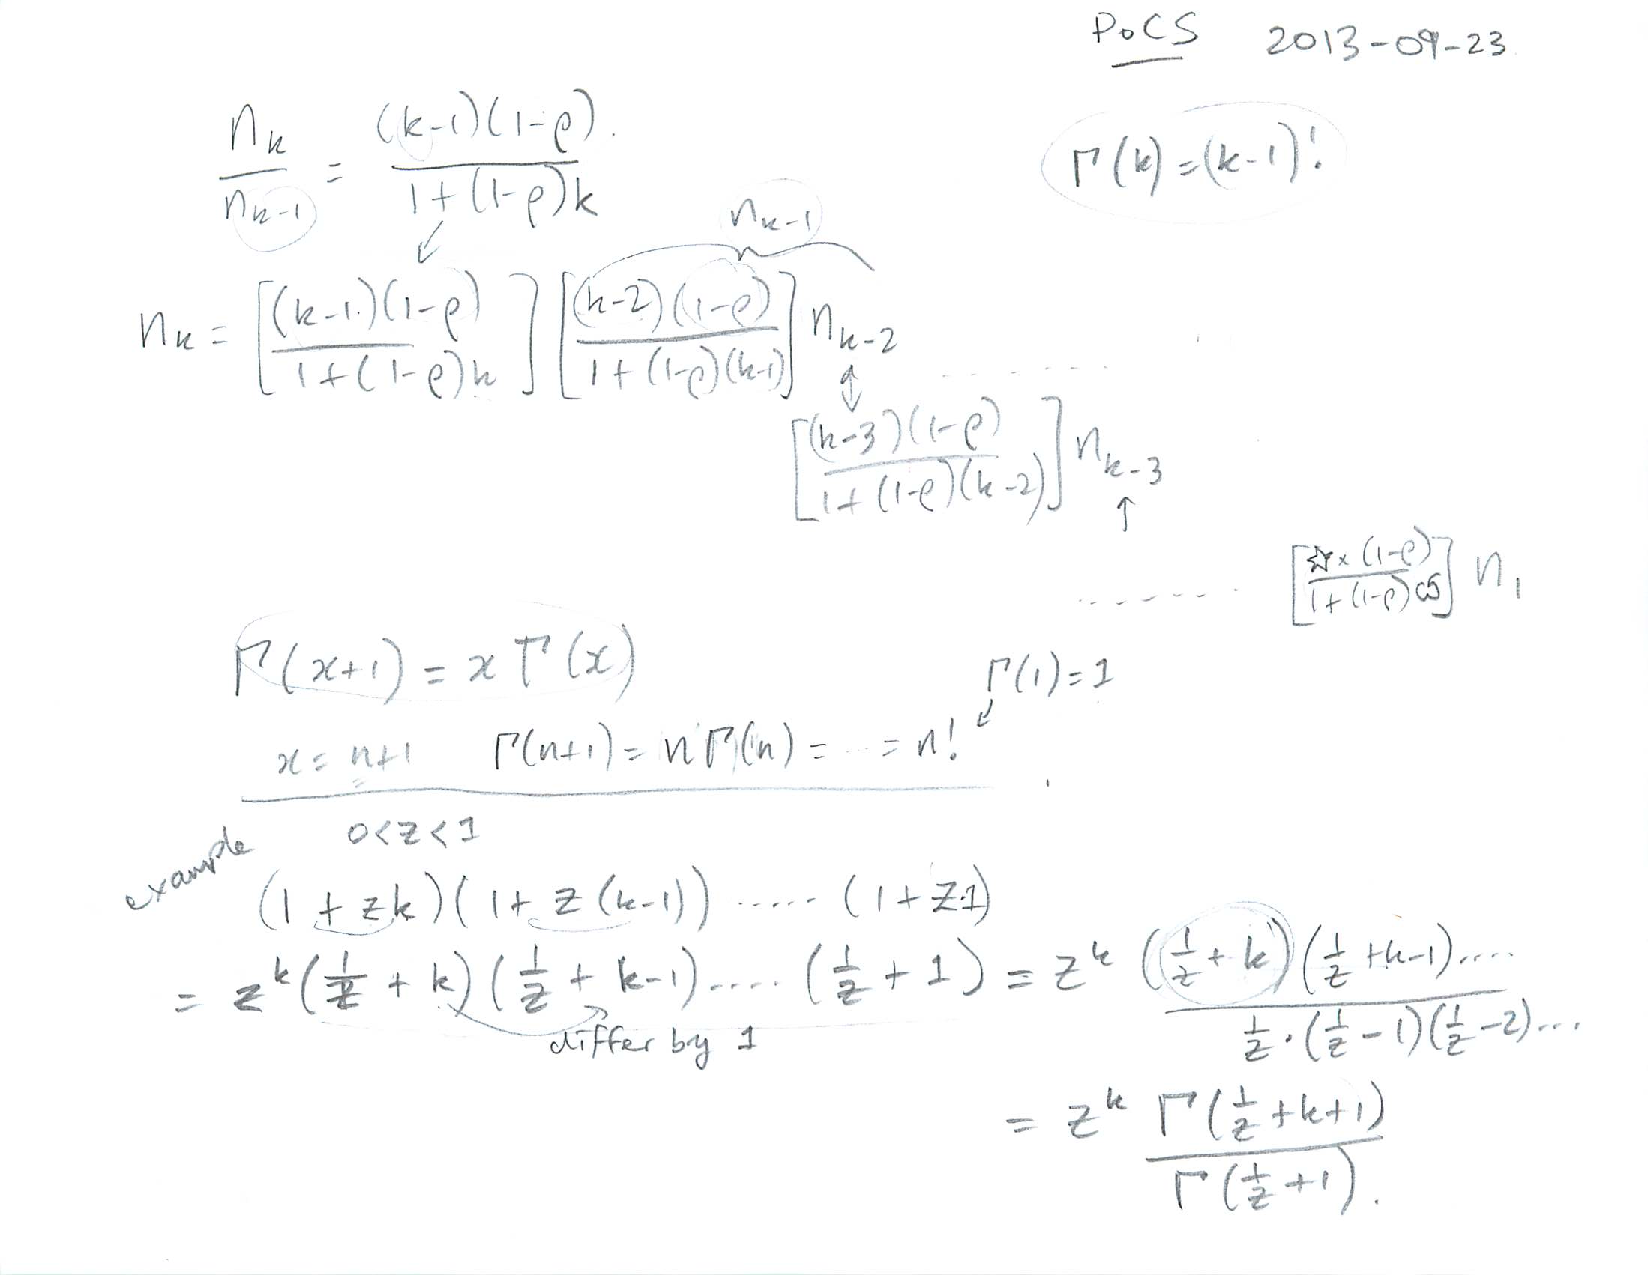
\includegraphics[width=\linewidth]{2013-09-23pocs-assignment-help-gamma-functions-simons-model.pdf}
  }

  
   \solutionstart

   %% solution goes here

   \solutionend

\item 
  What happens to $\gamma$ in the limits $\simonalpha \rightarrow 0$
  and $\simonalpha \rightarrow 1$?  Explain in a sentence or 
  two what's going on in these cases and how the specific limiting
  value of $\gamma$ makes sense.

  
   \solutionstart

   %% solution goes here

   \solutionend

\item (6 + 3 + 3 points)

  In Simon's original model, the expected total number of distinct
  groups at time $t$ is $\simonalpha t$.
  Recall that each group is made up of elements of a particular flavor.

  In class, we derived the fraction of groups containing
  only 1 element, finding
  $$
  n^{(g)}_1 =
  \frac{
    N_{1}(t)}
       {\simonalpha t}
       = \frac{1}{2-\simonalpha}
       $$

       \begin{enumerate}
       \item (3 + 3 points)

         Find the form of $n^{(g)}_2$ and $n^{(g)}_3$,
         the fraction of groups that are of size 2 and size 3.
         
         
   \solutionstart

   %% solution goes here

   \solutionend

       \item 
         Using data for James Joyce's Ulysses (see below), 
         first show that Simon's estimate for
         the innovation rate $\simonalpha_{\rm est} \simeq 0.115$
         is reasonably accurate for the version of the text's word counts
         given below.
         
         Hint: You should find a slightly higher number
         than Simon did.

         Hint: Do not compute $\simonalpha_{\rm est}$ from
         an estimate of $\gamma$.

         %% You should find $\simonalpha_{\rm est} \simeq 0.119$.

         
   \solutionstart

   %% solution goes here

   \solutionend
         

       \item
         Now compare the theoretical estimates
         for $n^{(g)}_1$, $n^{(g)}_2$, and $n^{(g)}_3$,
         with empirical values you obtain for Ulysses.

         
   \solutionstart

   %% solution goes here

   \solutionend

       \end{enumerate}

       The data (links are clickable):
       \begin{itemize}
       \item 
         Matlab file (\texttt{sortedcounts} = word frequency $f$ in descending order, \texttt{sortedwords} = ranked words):\\
         \href{\coursewebsite/docs/ulysses.mat}{\coursewebsitetext/docs/ulysses.mat}
       \item
         Colon-separated text file (first column = word, second column = word frequency $f$):\\
         \href{\coursewebsite/docs/ulysses.txt}{\coursewebsitetext/docs/ulysses.txt}
       \end{itemize}

       Data taken from
       \wordwikilink{http://www.doc.ic.ac.uk/~rac101/concord/texts/ulysses/}{http://www.doc.ic.ac.uk/$\sim$rac101/concord/texts/ulysses/}.
       
       Note that some matching words with differing capitalization are recorded as separate words.

     \item (3 + 3)

       Repeat the preceding data analysis for Ulysses for Jane Austen's ``Pride
       and Prejudice'' and Alexandre Dumas' ``Le comte de Monte-Cristo'' (in
       the original French), working this time from the original texts.

       For each text, measure the fraction of words that appear only once, twice, and three times,
       and compare them with the theoretical values offered by Simon's model.
       
       Download text (UTF-8) versions from \wordwikilink{https://www.gutenberg.org}{https://www.gutenberg.org}:
       \begin{itemize}
       \item
         Pride and Prejudice:
         \wordwikilink{https://www.gutenberg.org/ebooks/42671}{https://www.gutenberg.org/ebooks/42671}.
       \item
         Le comte de Monte-Cristo:
         \wordwikilink{https://www.gutenberg.org/ebooks/17989}{https://www.gutenberg.org/ebooks/17989}.
       \end{itemize}

       You will need to parse and count words using your favorite/most-hated language
       (Python, R, Perl-ha-ha, etc.).

       Gutenberg adds some (non-uniform) boilerplate to the beginning and
       ends of texts, and you should remove that first.  Easiest to do so
       by inspection for just two texts.

       For a curated version of Gutenberg, see this paper by Gerlach and Font-Clos:
       \wordwikilink{https://arxiv.org/abs/1812.08092}{https://arxiv.org/abs/1812.08092}.

       
   \solutionstart

   %% solution goes here

   \solutionend

       



\end{enumerate}
